\documentclass[11pt]{article}

% for images
\usepackage{graphicx}
\graphicspath{{img/}}
% for affiliation on title page
\usepackage{authblk}
% for source in images
\usepackage{floatrow}
% for urls
\usepackage{url}
% for references
\usepackage{biblatex}
\addbibresource{references.bib}

\begin{document}

\title{Deep learning classification of rheumatoid arthritis}
\author{Janick Rohrbach}
\affil{Zurich University of Applied Sciences, School of Engineering, Institute of Data Analysis and Process Design (IDP)}
\maketitle

\newpage
	
\begin{abstract}
....
\end{abstract}

\newpage

\section{Introduction}
\label{sec:intro}


\subsection{Rheumatoid arthritis}
\label{subsec:rheuma}

Rheumatoid arthritis is caused by a malfunctioning immune system. The immune attacks healthy tissue instead of bacteria and viruses. This causes inflammation in the joints. Irreversible damage to the joint can occur, if the inflammation lasts for a long time. \cite{rheuma}


\begin{figure}
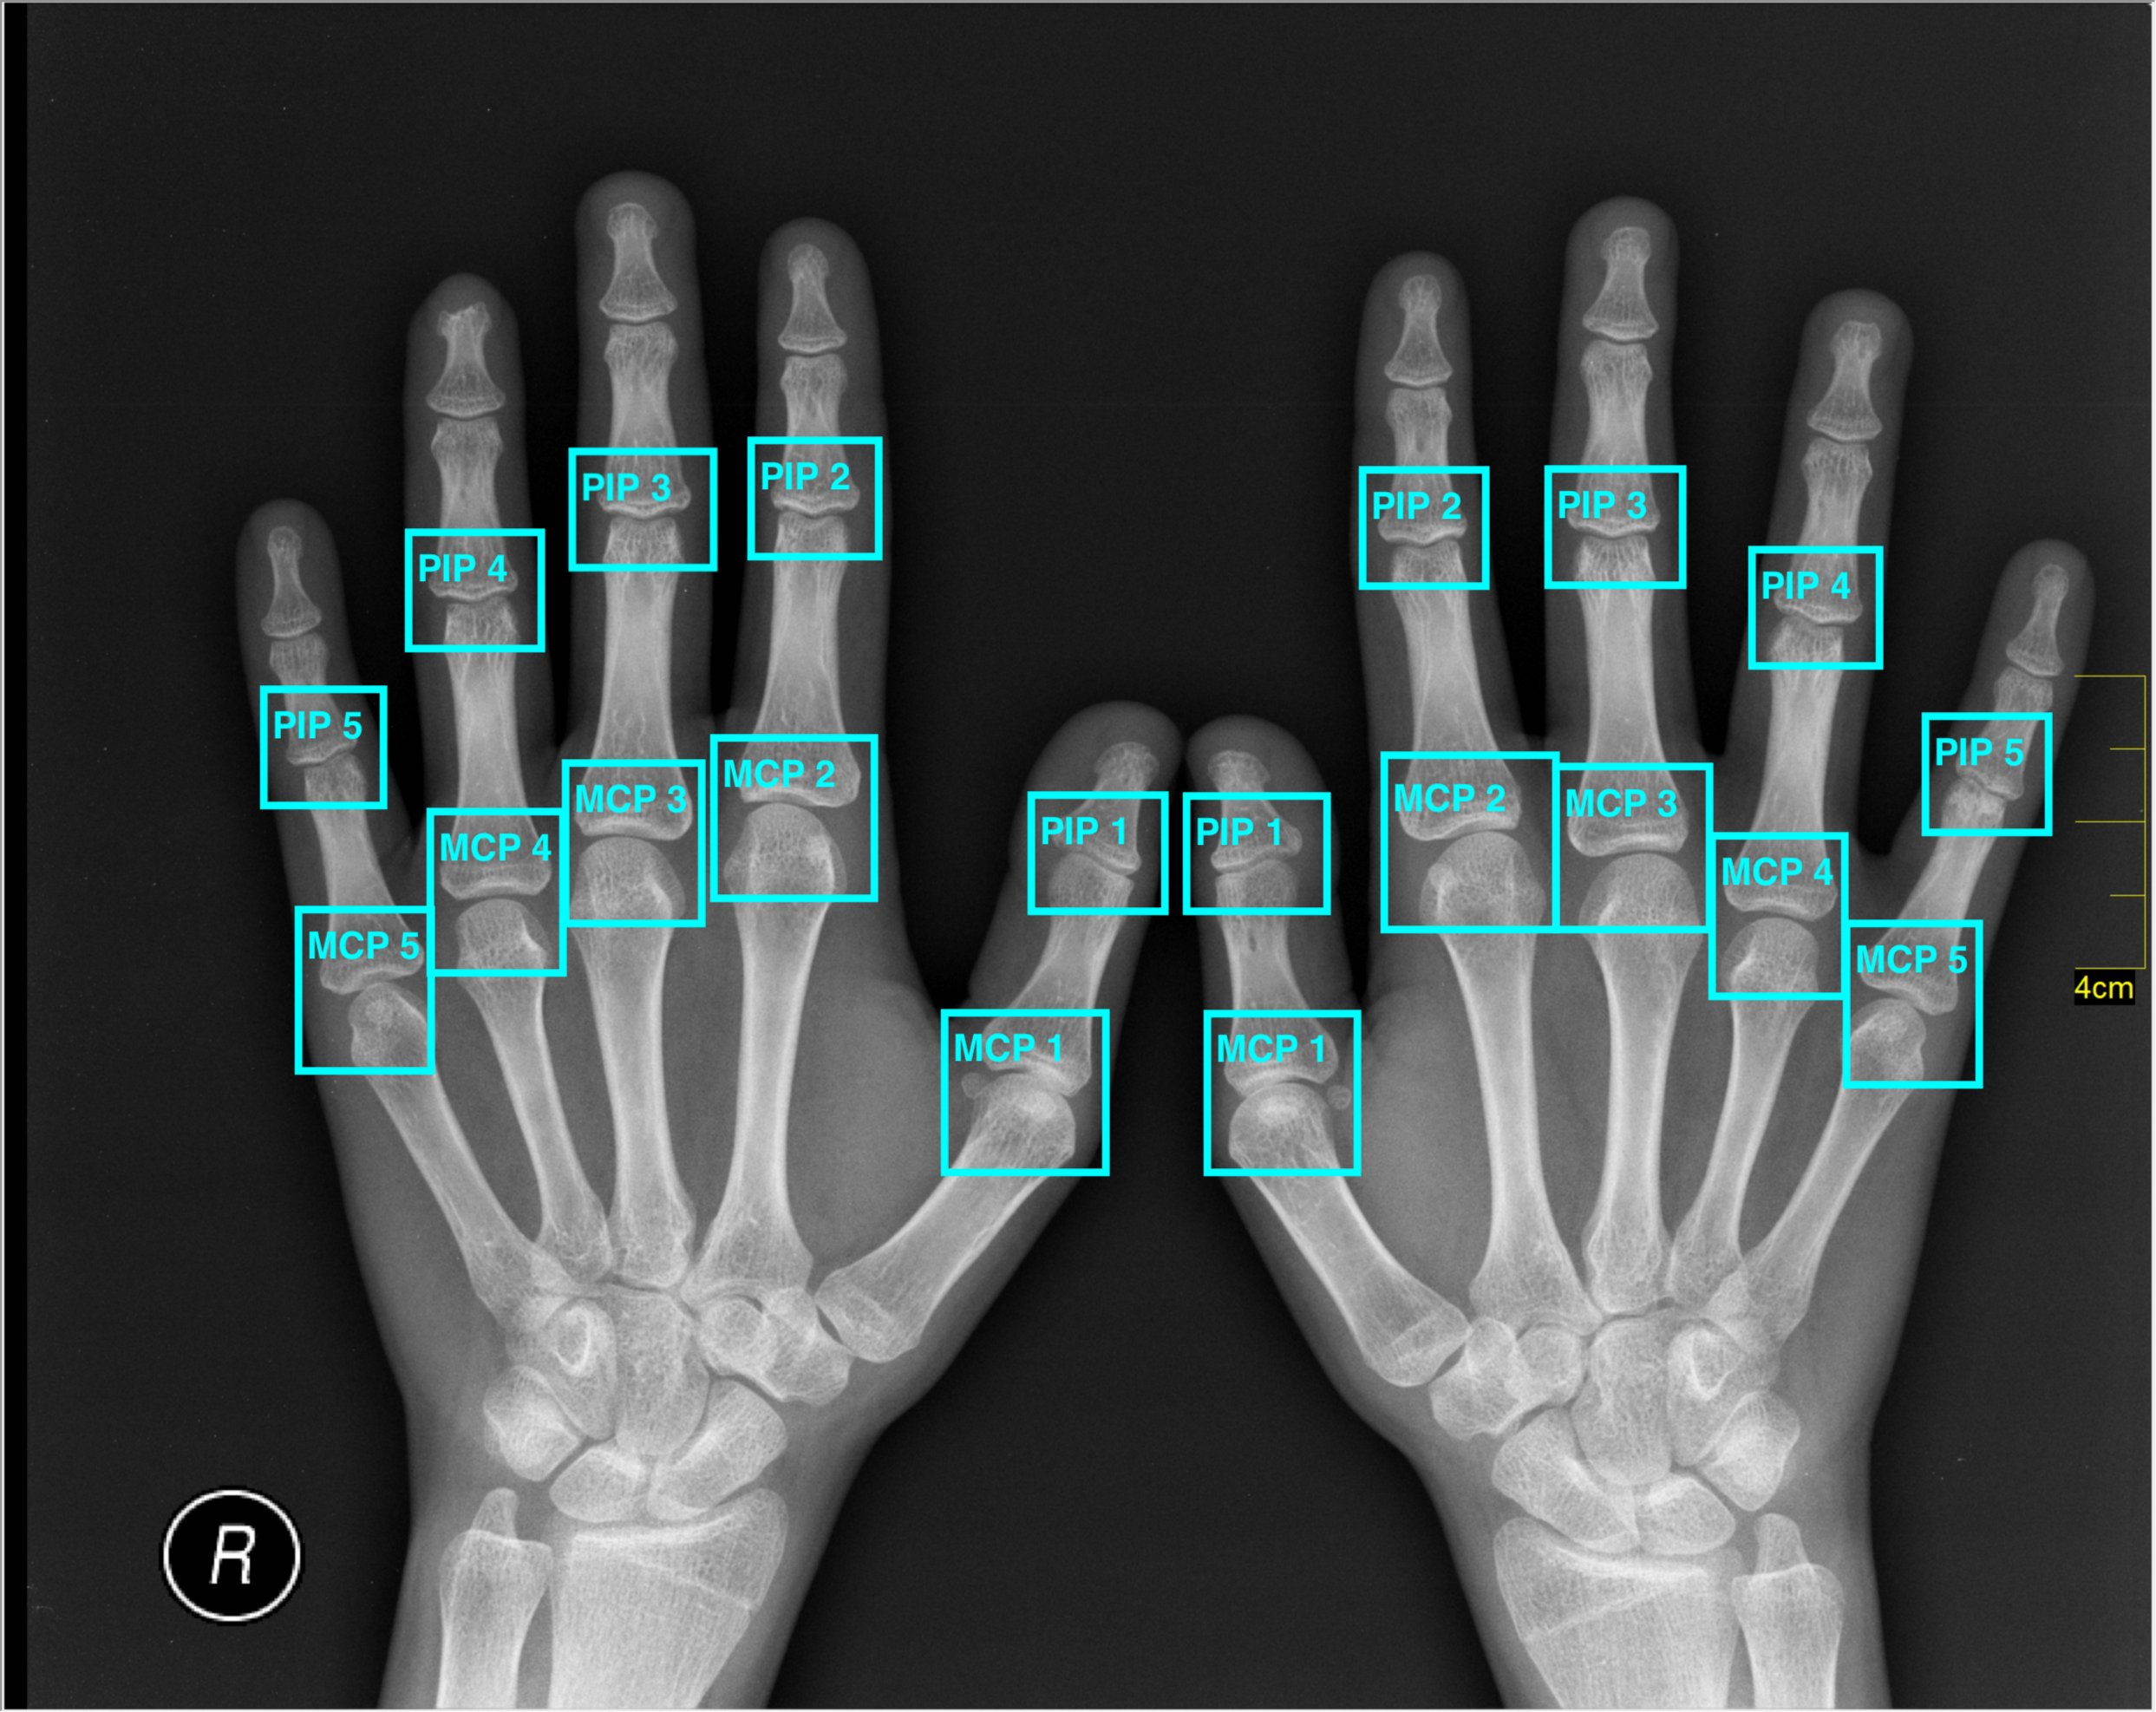
\includegraphics[width=10cm]{labels}	
\caption{Proximal interphalangeal joints (PIP) and carpometacarpal joints (MCP).}
\floatfoot{Image by Nevit Dilmen (CC BY-SA) \url{https://commons.wikimedia.org/wiki/File:Medical\_X\-Ray\_imaging\_OPC06\_nevit.jpg}}
\label{fig:labels}
\end{figure}

\subsection{Convolutional neural networks}
\label{subsec:cnn}
Convolutional neural networks take an image as an input. The image then gets passed through several convolutional layers. These layers work as filters and detect different features in the image. The weights of these layers are combined to class scores. Andrey Karpathy provides a good overview over convolutional neural networks in his course notes for the Stanford class CS231n. \cite{cnn}





\newpage
\section*{References}

\printbibliography

\newpage
\listoffigures


\end{document}
